\documentclass[12pt,a4paper,twoside,openright,titlepage,final]{article}
\usepackage{fontspec}
\usepackage{amsmath}
\usepackage{amsfonts}
\usepackage{amssymb}
\usepackage{makeidx}
\usepackage{graphicx}
\usepackage[hidelinks,unicode=true]{hyperref}
\usepackage[spanish,es-nodecimaldot,es-lcroman,es-tabla,es-noshorthands]{babel}
\usepackage[left=3cm,right=2cm, bottom=4cm]{geometry}
\usepackage{natbib}
\usepackage{microtype}
\usepackage{ifdraft}
\usepackage{verbatim}
\usepackage[nottoc]{tocbibind}
\usepackage{pdflscape}
\usepackage{fancyvrb}
\usepackage[obeyDraft]{todonotes}
\ifdraft{
	\usepackage{draftwatermark}
	\SetWatermarkText{BORRADOR}
	\SetWatermarkScale{0.7}
	\SetWatermarkColor{red}
}{}
\usepackage{booktabs}
\usepackage{longtable}
\usepackage{calc}
\usepackage{array}
\usepackage{caption}
\usepackage{subfigure}
\usepackage{footnote}
\usepackage{url}
\usepackage[titletoc]{appendix}

\setsansfont[Ligatures=TeX]{texgyreadventor}
\setmainfont[Ligatures=TeX]{texgyrepagella}
\setmonofont{FreeMono}

\usetikzlibrary{decorations.pathreplacing}

%*******************************************************
%                 NO MODIFICAR
\newcommand*{\FSfont}[1]{%
  \fontencoding{T1}\fontfamily{#1}\selectfont}

\newlength{\tpheight}\setlength{\tpheight}{0.9\textheight}
\newlength{\txtheight}\setlength{\txtheight}{0.9\tpheight}
\newlength{\tpwidth}\setlength{\tpwidth}{0.9\textwidth}
\newlength{\txtwidth}\setlength{\txtwidth}{0.9\tpwidth}
\newlength{\drop}
%*******************************************************

% Crea una portada con los siguientes parámetros
%
% #1 : Título 
% #2 : Subtítulo
% #3 : Subsubtítulo
% #4 : Autor(es)
% #5 : Lugar
%

\newcommand*{\portada}[5]{
\begin{titlepage}
\begingroup
\vspace*{1cm}
\drop = 0.2\txtheight
\centering
\vfill
{\Huge \scshape #1}\\[\baselineskip]
{\Large \textbf{#2}}\\[\baselineskip]
{\Large \scshape #3}\\[\baselineskip]
\vspace*{0.3cm}
{\large \textit{#4}}\\[0.5\drop]

\includegraphics[scale=0.35]{./imagenes/logoURJC.jpg}
\vspace*{1.5cm}

{\large \scshape #5, \today} \par
\begin{center}
\end{center}
\vfill\null
\endgroup
\end{titlepage}
}
 %*****************************************************
 


\author{José Ignacio Escribano}

\title{}

\setlength{\parindent}{0pt}

\begin{document}

\pagenumbering{alph}
\setcounter{page}{1}

\portada{Trabajo final}{Análisis de Datos Avanzados}{Análisis de series temporales}{José Ignacio Escribano}{Móstoles}

\tableofcontents
\thispagestyle{empty}
\newpage

\listoffigures
\thispagestyle{empty}
\newpage

\listoftables
\thispagestyle{empty}
\newpage

\pagenumbering{arabic}
\setcounter{page}{1}

\section{Introducción}

En este caso práctico utilizaremos la metodología Box-Jenkins para analizar dos series temporales. La primera es el índice de empleo de un determinado país, y la segunda es el volumen de ventas mensual de puros de una empresa tabacalera. En ambos casos, se trata de obtener un modelo que se ajuste lo máximo posible a la serie temporal.\\

La metodología Box-Jenkins recoge los pasos necesarios para obtener el modelo más adecuado de serie temporal:

\begin{enumerate}
	\item Especificación inicial: consiste en determinar el orden de integración de la serie temporal y naturaleza de diferencias que se requerirán para convertir en estacionaria la serie temporal. En este paso se usa el análisis gráfico de la serie, además de los correlogramas simple y parcial de la serie. 
	Una vez hecho lo anterior, habrá que decidir los órdenes de los polinomios autorregresivo y de medias móviles. De nuevo, se hará uso del correlograma simple y parcial de la serie. La Tabla~\ref*{tbl:modelos} recoge las principales características de la función de autocorrelación y de autocorrelación parcial de los principales modelos estacionarios. 
	
	\begin{table}[htbp!]
		\centering
		\caption{Principales características de la función de autocorrelación y de autocorrelación parcial de los principales modelos estacionarios}
		\label{tbl:modelos}
		\begin{tabular}{@{}ccc@{}}
			\toprule
			\textbf{Modelo} & \textbf{\begin{tabular}[c]{@{}c@{}}Función de \\ autocorrelación\end{tabular}}                            & \textbf{\begin{tabular}[c]{@{}c@{}}Función de \\ autocorrelación parcial\end{tabular}}                      \\ \midrule
			AR(p)           & \begin{tabular}[c]{@{}c@{}}Decrecimiento rápido hacia cero, \\ sin llegar a anularse\end{tabular}         & \begin{tabular}[c]{@{}c@{}}$p$ primera autocorrelaciones distintas \\ de cero, y el resto cero\end{tabular} \\
			MA(q)           & \begin{tabular}[c]{@{}c@{}}$q$ primeras autocorrelaciones \\ significativas, y el resto cero\end{tabular} & \begin{tabular}[c]{@{}c@{}}Decrecimiento rápido hacia cero,\\ sin llegar a anularse\end{tabular}            \\
			ARMA(p,q)       & \begin{tabular}[c]{@{}c@{}}Decrecimiento rápido hacia cero, \\ sin llegar a anularse\end{tabular}           & \begin{tabular}[c]{@{}c@{}}Decrecimiento rápido hacia cero,\\ sin llegar a anularse\end{tabular}            \\ \bottomrule
		\end{tabular}
	\end{table}
	
	\item Estimación: en este paso, se procede a estimar los modelos propuestos, normalmente mediante máxima verosimilitud o mínimos cuadrados no lineales. 
	
	\item Chequeo o validación: en este paso, se validan los posibles modelos y se escoge el que parezca más adecuado para describir la serie temporal.
	
	\item Utilización del modelo: el modelo escogido se puede utilizar para predecir futuros valores de la serie, entre otras opciones.
\end{enumerate}

\section{Resolución de las series temporales}

A continuación, aplicamos la metodología Box-Jenkins para obtener un modelo que se adecue a cada una de las series temporales planteadas. 

\subsection{Índice de empleo de un determinado país}

La primera serie temporal es el índice de empleo de un determinado país. La serie está corregida de estacionalidad y tiene frecuencia trimestral. El período muestral abarca desde el primer trimestre del año 1962 hasta el cuarto trimestre del año 1994.\\

Comenzamos representando la serie temporal (Figura~\ref{fig:empleo}).

\begin{figure}[tbph!]
\centering
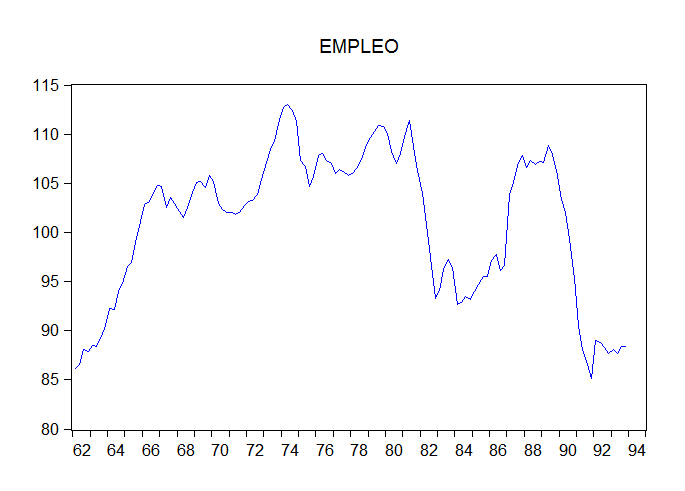
\includegraphics[width=0.8\linewidth]{imagenes/empleo/empleo.png}
\caption{Serie temporal empleo}
\label{fig:empleo}
\end{figure}

Se observa que podría haber tendencia en la serie original. Para verificarlo, usamos el correlograma de la serie que se puede ver en la Figura~\ref{fig:correlograma-empleo}.\\
 
\begin{figure}[tbph!]
	\centering
	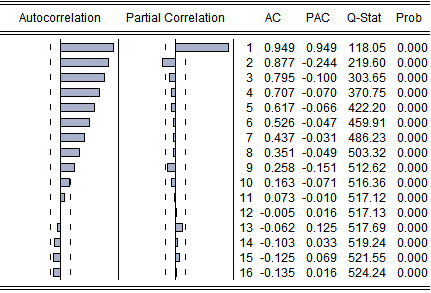
\includegraphics[width=0.7\linewidth]{imagenes/empleo/correlograma-empleo.png}
	\caption{Correlograma de la serie temporal empleo}
	\label{fig:correlograma-empleo}
\end{figure}

Como se observa un decrecimiento lento en la parte positiva del eje X, estamos ante una serie que presenta tendencia, por lo que estamos ante una serie no estacionaria. Tenemos que eliminar la tendencia, haciendo uso de las diferencias regulares de la serie original.\\

Tomamos la primera diferenciación para convertir la serie en estacionaria, que llamamos dempleo. Representamos la nueva serie para comprobar que hemos eliminado la tendencia de la serie original.  \\

\begin{figure}[tbph!]
	\centering
	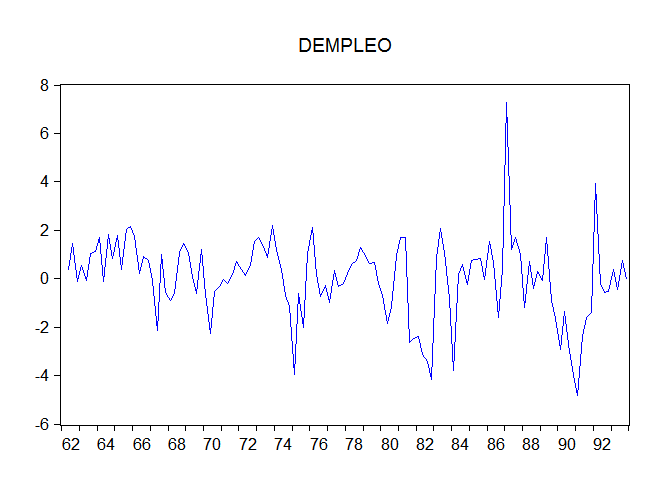
\includegraphics[width=0.8\linewidth]{imagenes/empleo/empleo-diferenciada.png}
	\caption{Serie transformada tomando una diferencia regular}
	\label{fig:empleo-diferenciada}
\end{figure}

La nueva serie parece indicar que estamos ante una serie estacionaria, ya que hemos eliminado la tendencia tomando una diferencia regular, y la serie carecía de estacionalidad de acuerdo al enunciado. Esto se puede comprobar mirando el correlograma de esta nueva serie (Figura~\ref{fig:correlograma-empleo-diferenciada}).\\ 

\begin{figure}[tbph!]
	\centering
	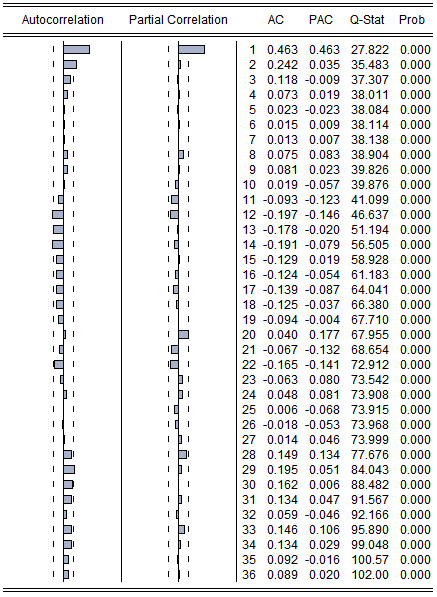
\includegraphics[width=0.7\linewidth]{imagenes/empleo/correlograma-empleo-diferenciada.png}
	\caption{Correlograma de la serie temporal transformada dempleo}
	\label{fig:correlograma-empleo-diferenciada}
\end{figure}

Así pues, tenemos que $d=1$ y $D=0$, y

\[ \text{dempleo} = (1-B) \text{empleo}\]

Es decir, dempleo es un modelo integrado de orden 1.\\

Observando el correlograma de la Figura~\ref{fig:correlograma-empleo-diferenciada} podemos sugerir que la serie temporal puede venir dada por un modelo AR(1), ya que la función de autocorrelación decrece rápidamente hacia cero, sin llegar a anularse, y en la función de autocorrelación parcial, hay un valor no nulo positivo, y el resto es cero. También podría tratarse de un modelo MA(2), ya que en la función de autocorrelación hay dos valores no nulos positivos y el resto es cero, y en la función de autocorrelación parcial hay un decrecimiento rápido sin llegar a anularse. Así planteamos los siguientes modelos:

\begin{enumerate}
	\item ARIMA(1,1,0) \label{mod:1}, que escrito en forma de ecuación es
	
	\[ (1-\theta_1 B) (1-B) \text{empleo} = a_t \] 
	\item ARIMA(0,1,2) \label{mod:2}, que escrito en forma de ecuación es
	
	\[ (1-\theta_1 B) (1-B) \text{empleo} = (1-\theta_1 B - \theta_2 B^2)a_t \] 
	\item ARIMA(1,1,2) \label{mod:3}, que escrito en forma de ecuación es
	
	\[ (1-B) \text{empleo} = (1-\theta_1 B - \theta_2 B^2) a_t \] 
\end{enumerate}

Estimamos cada uno de los modelos propuestos. En primer lugar estimamos el modelo ARIMA(1,1,0). La salida de EViews de este modelo se muestra en la Figura~\ref{fig:modelo1-estadisticas}.\\


\begin{figure}[tbph!]
	\centering
	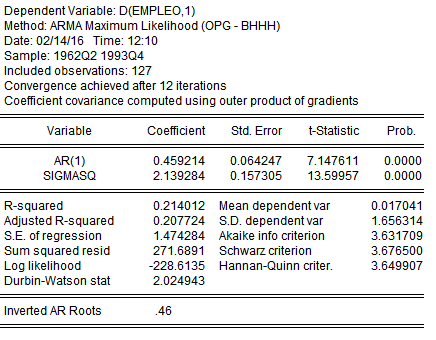
\includegraphics[width=0.7\linewidth]{imagenes/empleo/modelo1-estadisticas.png}
	\caption{Estimación del modelo ARIMA(1,1,0)}
	\label{fig:modelo1-estadisticas}
\end{figure}

Se observa que todos los parámetros del modelo son significativos, por lo que lo consideraremos adecuado. Además, se obtiene un valor de $R^2$ ajustado de 0.214.\\

Estimamos nuestro segundo modelo, es decir, el modelo ARIMA(0,1,2) usando EViews. La salida que produce este programa se puede ver en la Figura~\ref{fig:modelo2-estadisticas}.\\

\begin{figure}[tbph!]
	\centering
	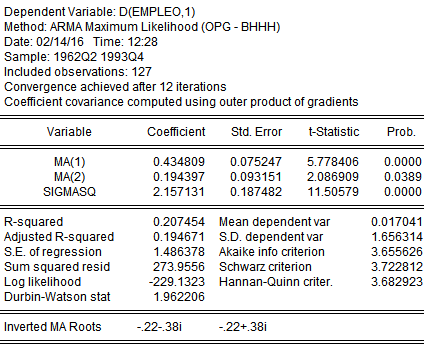
\includegraphics[width=0.7\linewidth]{imagenes/empleo/modelo2-estadisticas.png}
	\caption{Estimación del modelo ARIMA(1,1,2)}
	\label{fig:modelo2-estadisticas}
\end{figure}

Observando la salida de EViews, tenemos que todos los parámetros del modelo son significativos, por lo que consideraremos este modelo adecuado para representar la serie de tiempo del índice de empleo. Además, tiene tiene un coeficiente $R^2$ ajustado de 0.195.\\

Por último, estimamos nuestro último modelo propuesto: el ARIMA(1,1,2). De nuevo, usamos EViews que nos devuelve la salida de la Figura~\ref{fig:modelo3-estadisticas}.\\

\begin{figure}[tbph!]
	\centering
	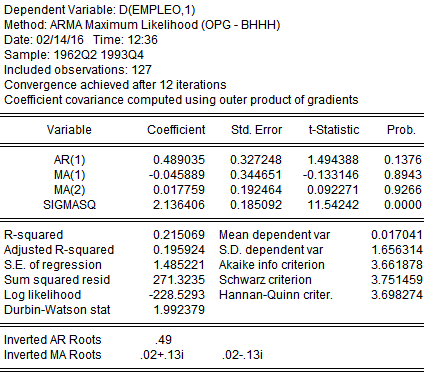
\includegraphics[width=0.7\linewidth]{imagenes/empleo/modelo3-estadisticas.png}
	\caption{Estimación del modelo ARIMA(0,1,2)}
	\label{fig:modelo3-estadisticas}
\end{figure}

Observando la salida de este modelo, vemos que todos los parámetros no son significativos, por lo que desechamos este modelo ya que no parece adecuado para describir la serie temporal que estamos tratando.\\

Sólo tenemos dos modelos que validar: el modelo ARIMA(1,1,0) y el ARIMA(0,1,2). La Tabla~\ref{tbl:empleo-estadisticas} muestra una comparativa entre la estimación de los dos modelos.\\

\begin{table}[htbp!]
	\centering
	\caption{Análisis de la estimación de los modelos ARIMA(1,1,0) y ARIMA(0,1,2)}
	\label{tbl:empleo-estadisticas}
	\begin{tabular}{@{}ccc@{}}
		\toprule
		\textbf{}                                                       & \textbf{ARIMA(1,1,0)} & \textbf{ARIMA(0,1,2)} \\ \midrule
		$R^2$                                                           & $0.214$               & $0.207$               \\
		$R^2$ ajustado                                                  & $0.208$               & $0.195$               \\
		\begin{tabular}[c]{@{}c@{}}Akaike Info\\ Criterion\end{tabular} & $3.631$               & $3.656$               \\
		\begin{tabular}[c]{@{}c@{}}Schwarz\\ Criterion\end{tabular}     & $3.677$               & $3.723$               \\
		\begin{tabular}[c]{@{}c@{}}Error de\\ regresión\end{tabular}    & $1.474$               & $1.487$               \\ \bottomrule
	\end{tabular}
\end{table} 

El modelo ARIMA(1,1,0) tiene un menor error (1.474) que el modelo ARIMA(0,1,2) (1.487). Además tanto los estadísticos de Akaike como de Scharwz son menores en el modelo ARIMA(1,1,0) que en el modelo ARIMA(0,1,2). Lo anterior parece indicar que el modelo más adecuado es el ARIMA(1,1,0).\\

Para confirmar nuestras sospechas, hacemos un análisis de los residuos de ambos modelos. \\

Comenzamos con el modelo ARIMA(1,1,0). En la Figura~\ref*{fig:modelo1-residuos-correlograma} se puede ver el correlograma de los residuos del modelo.\\

\begin{figure}[tbph!]
	\centering
	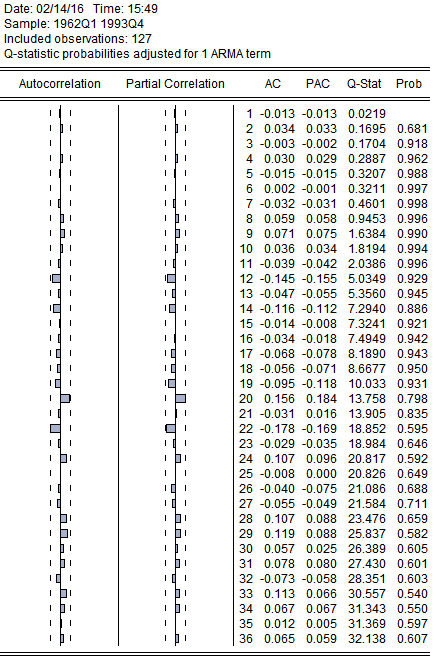
\includegraphics[width=0.7\linewidth]{imagenes/empleo/modelo1-residuos-correlograma.png}
	\caption{Correlograma de los residuos del modelo ARIMA(1,1,0)}
	\label{fig:modelo1-residuos-correlograma}
\end{figure}

Se puede observar que las autocorrelaciones de los residuos no son significativas y entran dentro de las bandas de confianza, lo que indica que no son distintas de cero. De la misma forma, el estadístico Q no muestra indicios de autocorrelación de los residuos, por lo que todo parece indicar que estamos ante ruido blanco. Para comprobarlo, representamos el gráfico de residuos, que se puede ver en la Figura~\ref{fig:modelo1-residuos}.\\

\begin{figure}[tbph!]
	\centering
	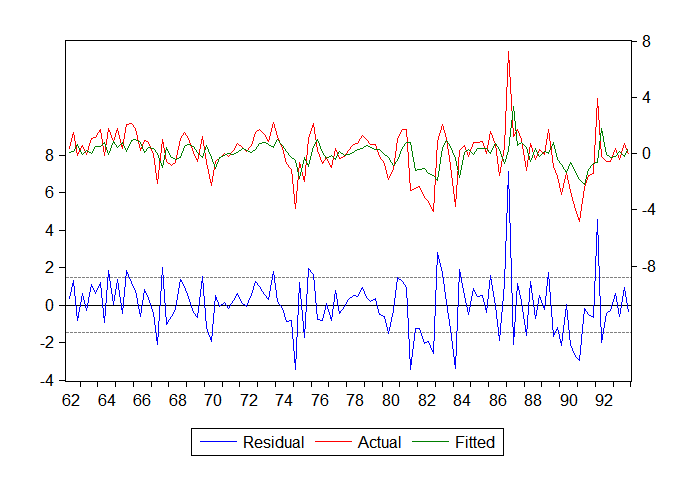
\includegraphics[width=0.7\linewidth]{imagenes/empleo/modelo1-residuos.png}
	\caption{Residuos del modelo ARIMA(1,1,0)}
	\label{fig:modelo1-residuos}
\end{figure}

La mayoría de los residuos se encuentran dentro de las bandas de confianza, lo que apoya la teoría de autocorrelación. Todo parece confirmar que los residuos se comportan como ruido blanco, es decir, tienen media 0 y varianza constante.\\

Notar la presencia de un outlier en el primer trimestre de 1987.\\

Procedemos de forma similar para comprobar que los residuos del modelo son ruido blanco.\\

Las Figuras~\ref{fig:modelo2-residuos-correlograma}~y~\ref{fig:modelo2-residuos} muestran la presencia de los residuos como ruido blanco.\\ 
 
\begin{figure}[tbph!]
	\centering
	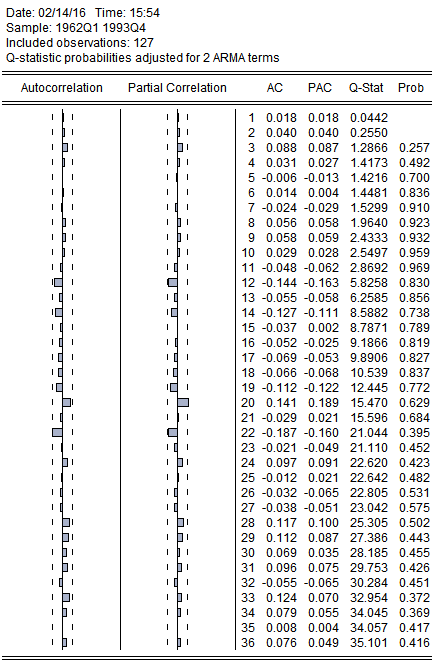
\includegraphics[width=0.7\linewidth]{imagenes/empleo/modelo2-residuos-correlograma.png}
	\caption{Correlograma de los residuos del modelo ARIMA(0,1,2)}
	\label{fig:modelo2-residuos-correlograma}
\end{figure}

\begin{figure}[tbph!]
	\centering
	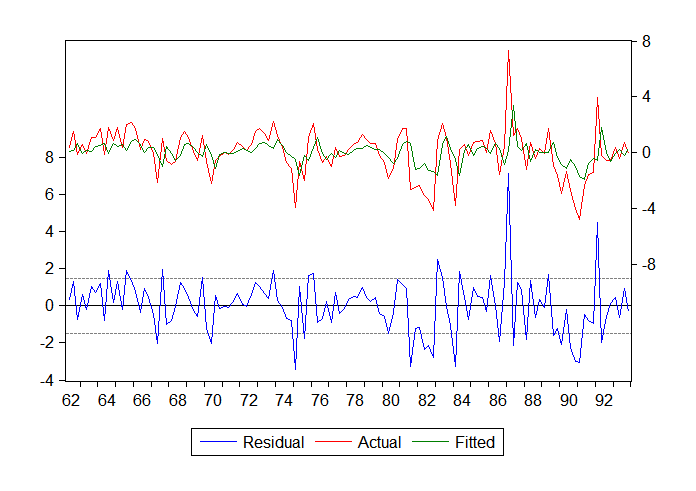
\includegraphics[width=0.7\linewidth]{imagenes/empleo/modelo2-residuos.png}
	\caption{Residuos del modelo ARIMA(0,1,2)}
	\label{fig:modelo2-residuos}
\end{figure}

De todo lo anterior, se deduce que el modelo ARIMA(1,1,0) es superior al modelo ARIMA(0,1,2) ya que tiene mejor coeficiente $R^2$, menor error en la estimación, y menores valores en los estadísticos de Akaike y Schwarz.\\

Así pues, el índice de empleo viene dado por el modelo ARIMA(1,1,0).\\

Utilizaremos este modelo para predecir los valores de empleo del año siguiente (1994). Los datos para cada uno de los trimestres se pueden ver en la Tabla~\ref{tbl:empleo-predicciones}.\\

 \begin{table}[htbp!]
 	\centering
 	\caption{Predicciones del índice de empleo para el año 1994}
 	\label{tbl:empleo-predicciones}
 	\begin{tabular}{@{}cc@{}}
 		\toprule
 		\textbf{Trimestre} & \textbf{Predicción} \\ \midrule
 		1/1994             & $88.34407$          \\
 		2/1994             & $88.33593$          \\
 		3/1994             & $88.33219$          \\
 		4/1994             & $88.33048$          \\ \bottomrule
 	\end{tabular}
 \end{table}

Según estas predicciones, el índice de empleo del 1994 se mantuvo constante, en torno al 88\%. 


\clearpage

\subsection{Venta de cigarros puros de una empresa tabacalera}

La segunda serie temporal es el volumen de ventas mensual de puros de una empresa tabacalera. El período de la serie abarca desde enero de 1989 hasta diciembre de 1996.\\

Comenzamos representando la serie temporal (Figura~\ref{fig:empleo}).\\

\begin{figure}[tbph!]
	\centering
	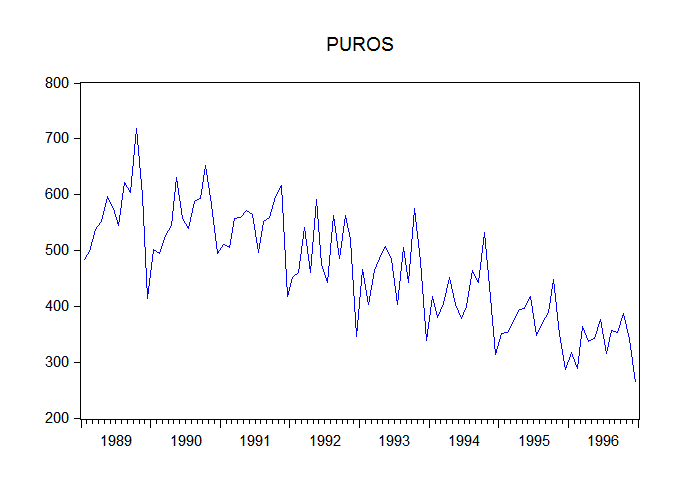
\includegraphics[width=0.8\linewidth]{imagenes/puros/puros.png}
	\caption{Serie temporal puros}
	\label{fig:puros}
\end{figure} 

Se puede ver una fuerte tendencia decreciente a lo largo de la serie temporal. Además, se observa una estacionalidad de los datos: la venta aumenta entre los meses de enero y septiembre, y desciende en los meses de octubre a diciembre.\\

Nos aseguramos de la presencia de tendencia y estacionalidad mirando el correlograma de la serie (Figura~\ref{fig:correlograma-puros}).\\

\begin{figure}[tbph!]
	\centering
	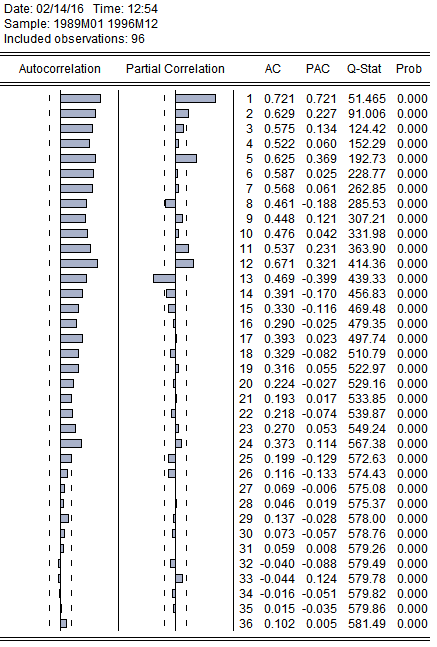
\includegraphics[width=0.8\linewidth]{imagenes/puros/correlograma-puros.png}
	\caption{Correlograma de la serie temporal puros}
	\label{fig:correlograma-puros}
\end{figure}

Se observa el decaimiento tanto en la parte regular como en la parte estacional, es decir, en los retardos múltiplos de 12, por lo que necesitamos eliminar la tendencia y la estacionalidad para que nuestra serie sea estacionaria.\\

Comenzamos eliminando la tendencia. Para ello, tomamos una diferencia regular de la serie, que llamaremos dpuros. La Figura~\ref{fig:puros-diferenciada} muestra nuestra nueva serie con una diferencia regular.\\

\begin{figure}[tbph!]
	\centering
	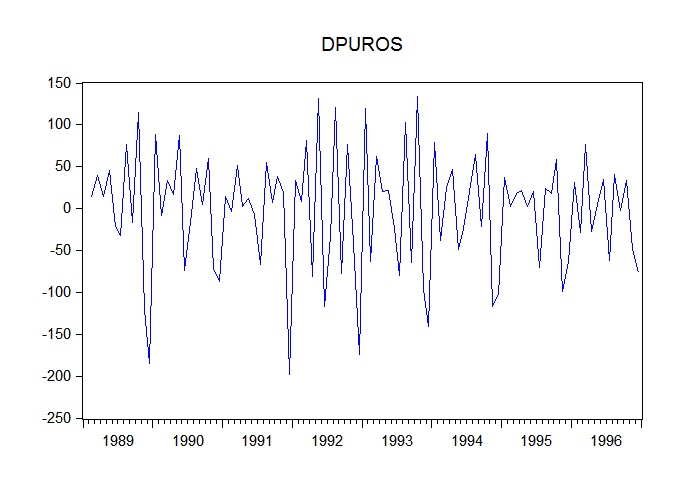
\includegraphics[width=0.8\linewidth]{imagenes/puros/puros-diferenciada.png}
	\caption{Serie temporal puros}
	\label{fig:puros-diferenciada}
\end{figure}

Observamos que se ha eliminado la tendencia, pero no así la estacionalidad. Para asegurarnos observamos de nuevo el correlograma de esta nueva serie temporal (Figura~\ref{fig:correlograma-puros-diferenciada}).\\


\begin{figure}[tbph!]
	\centering
	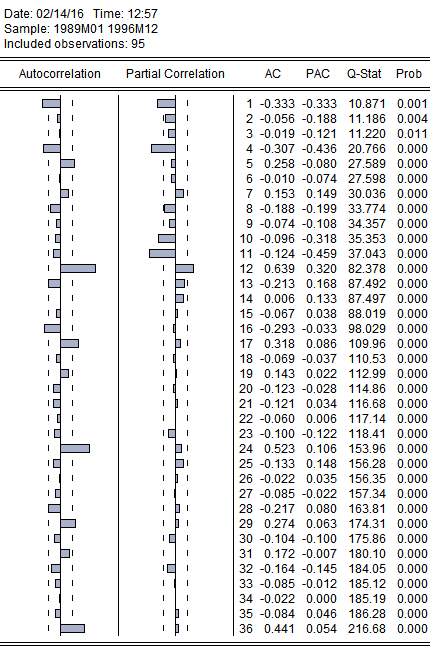
\includegraphics[width=0.8\linewidth]{imagenes/puros/correlograma-puros-diferenciada.png}
	\caption{Correlograma de la serie temporal diferenciada dpuros}
	\label{fig:correlograma-puros-diferenciada}
\end{figure}

En el correlograma se puede observar que se ha corregido la tendencia, pero no la estacionalidad en los retardos múltiplos de 12. Así que tomamos una diferencia estacional de período estacional 12. A esta nueva variable la llamamos ddpuros12, que se muestra en la Figura~\ref{fig:puros-diferenciada-estacional12}.\\

\begin{figure}[tbph!]
	\centering
	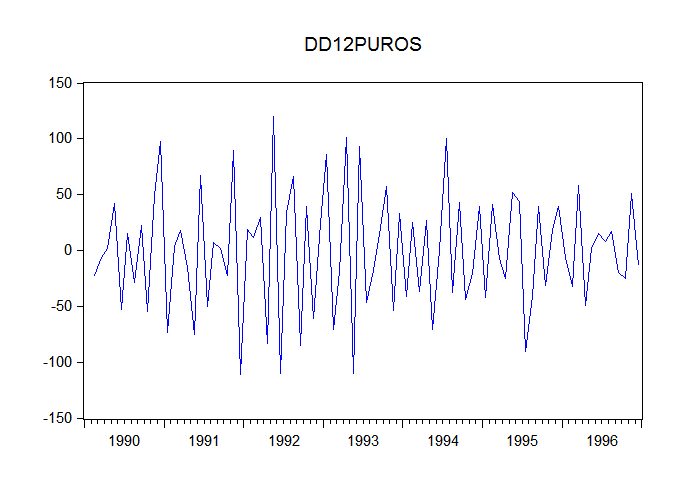
\includegraphics[width=0.8\linewidth]{imagenes/puros/puros-diferenciada-estacional12.png}
	\caption{Serie temporal ddpuros12}
	\label{fig:puros-diferenciada-estacional12}
\end{figure}

Se puede ver que esta nueva serie tiene tanto ausencia de tendencia como de estacionalidad. Para asegurarnos, vemos el correlograma de esta serie (Figura~\ref{fig:correlograma-puros-diferenciada-estacional12}).\\

\begin{figure}[tbph!]
	\centering
	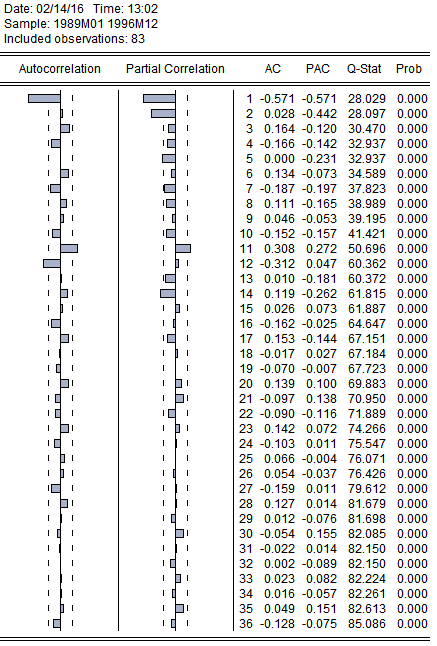
\includegraphics[width=0.8\linewidth]{imagenes/puros/correlograma-puros-diferenciada-estacional12.png}
	\caption{Correlograma de la serie temporal ddpuros12}
	\label{fig:correlograma-puros-diferenciada-estacional12}
\end{figure}

El correlograma no deja duda de que esta nueva serie es estacionaria.\\

Por tanto, para convertir la serie en estacionaria hemos tenido que aplicar la siguiente transformación:

\[ \text{ddpuros12} = (1-B)(1-B^{12}) \cdot \text{puros} \]

Es decir, tenemos que $d=D=1$.\\

Debemos establecer el modelo generador de la serie.\\

El correlograma de la Figura~\ref{fig:correlograma-puros-diferenciada-estacional12} sugiere que el modelo puede estar generado por un MA(1) estacional ya que la función de autocorrelación presenta un valor no nulo en parte negativa del eje X en los múltiplos de 12 retardos, y la función de autocorrelación parcial muestra un decrecimiento lento en la parte negativa del eje X.\\

En la parte regular, el modelo puede estar dado por un AR(2), ya que la función de autocorrelación muestra un decrecimiento lento a lo largo de todos los retardos, y la función de autocorrelación parcial, dos valores no nulos negativos en la parte del eje X. También puede ser generado por un MA(1) ya que la función de autocorrelación presenta un valor no nulo negativo en el eje X, y la función de autocorrelación parcial presenta un decrecimiento lento en todos los retardos.\\

Así, los modelos candidatos a generar la serie son:

\begin{enumerate}
	\item ARIMA$(0,1,1)\times(0,1,1)_{12}$, que escrito en forma de ecuación es
	
	\[ (1-B) (1-B^{12}) \text{puros} = (1-\theta_1 B)(1-\Theta_{1}B^{12}) a_t \] 
	\item ARIMA$(2,1,0)\times(0,1,1)_{12}$, que escrito en forma de ecuación es
	
	\[ (1-\phi_1 B - \phi_2 B^2)(1-B) (1-B^{12}) \text{puros} = (1-\theta_{1}B^{12}) a_t \] 
\end{enumerate}

Necesitamos estimar ambos modelos y validarlos.\\

Comenzamos con el modelo ARIMA$(0,1,1)\times(0,1,1)_{12}$. En la Figura~\ref{fig:modelo1-puros} se muestra el resultado de la estimación de este modelo en EViews.\\

\begin{figure}[tbph!]
	\centering
	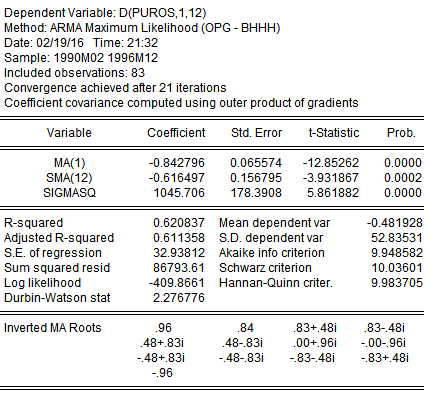
\includegraphics[width=0.8\linewidth]{imagenes/puros/modelo1.png}
	\caption{Estimación del modelo ARIMA$(0,1,1)\times(0,1,1)_{12}$}
	\label{fig:modelo1-puros}
\end{figure}

Se puede observar que todos los términos son significativos, y que tiene un coeficiente $R^2$ ajustado de 0.620.\\

Si ahora estimamos el modelo 2, es decir, el modelo ARIMA$(2,1,0)\times(0,1,1)_{12}$, se tiene el resultado de la Figura~\ref{fig:modelo2-puros}.\\

\begin{figure}[tbph!]
	\centering
	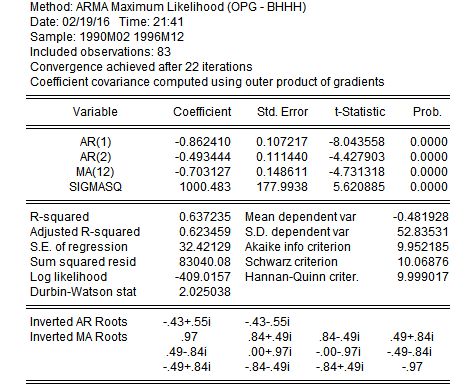
\includegraphics[width=0.8\linewidth]{imagenes/puros/modelo2.png}
	\caption{Estimación del modelo ARIMA$(2,1,0)\times(0,1,1)_{12}$}
	\label{fig:modelo2-puros}
\end{figure}

Se puede observar que todos los coeficientes de este modelo son significativos, y que tiene un coeficiente $R^2$ ajustado de 0.623.\\

A continuación, validaremos el modelo comparando tanto los resultados de la estimación como los residuos de ambos modelos. En la Tabla~\ref{tbl:puros-estadisticas} se puede ver una comparativa entre ambos modelos.\\

\begin{table}[htbp!]
	\centering
	\caption{Análisis de la estimación de los modelos ARIMA$(0,1,1)\times(0,1,1)_{12}$
	y ARIMA$(2,1,0)\times(0,1,1)_{12}$}
	\label{tbl:puros-estadisticas}
	\begin{tabular}{@{}ccc@{}}
		\toprule
		\textbf{}                                                       & \textbf{ ARIMA$(2,1,0)\times(0,1,1)_{12}$} & \textbf{ARIMA$(0,1,1)\times(0,1,1)_{12}$} \\ \midrule
		$R^2$                                                           & $0.620$               & $0.637$               \\
		$R^2$ ajustado                                                  & $0.611$               & $0.623$               \\
		\begin{tabular}[c]{@{}c@{}}Akaike Info\\ Criterion\end{tabular} & $9.949$               & $9.952$               \\
		\begin{tabular}[c]{@{}c@{}}Schwarz\\ Criterion\end{tabular}     & $10.036$               & $10.068$               \\
		\begin{tabular}[c]{@{}c@{}}Error de\\ regresión\end{tabular}    & $32.938$               & $32.421$               \\ \bottomrule
	\end{tabular}
\end{table} 

Se puede observar que el valor de los coeficientes $R^2$ y $R^2$ ajustado son mayores en el modelo ARIMA$(2,1,0)\times(0,1,1)_{12}$ que en el modelo ARIMA$(2,1,0)\times(0,1,1)_{12}$. Además, también es menor tanto el Akaike Info Criterion como el Schwarz Criterion en el modelo ARIMA$(2,1,0)\times(0,1,1)_{12}$. Sin embargo, el modelo ARIMA$(2,1,0)\times(0,1,1)_{12}$ tiene un menor error de regresión que el modelo ARIMA$(0,1,1)\times(0,1,1)_{12}$.\\

A continuación, pasamos a analizar los residuos de los modelos. Comenzamos con el modelo ARIMA$(0,1,1)\times(0,1,1)_{12}$. Las Figuras~\ref{fig:modelo1-puros-residuos}~y~\ref{fig:modelo1-puros-residuos-correlograma} muestra los residuos y el correlograma de estos. Se puede observar que la mayoría caen dentro de las bandas de confianza, por lo que es de suponer que los residuos se comportan como ruido blanco. El correlograma parece también contrastarlo.\\

\begin{figure}[tbph!]
	\centering
	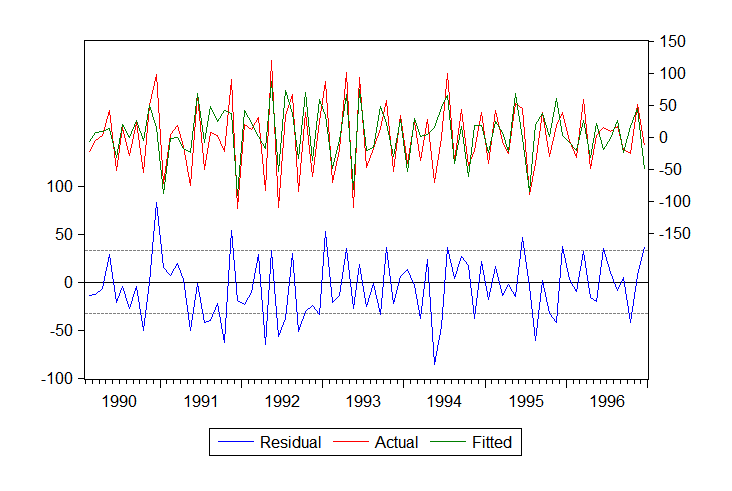
\includegraphics[width=0.8\linewidth]{imagenes/puros/modelo1-residuos.png}
	\caption{Residuos del modelo ARIMA$(0,1,1)\times(0,1,1)_{12}$}
	\label{fig:modelo1-puros-residuos}
\end{figure}

\begin{figure}[tbph!]
	\centering
	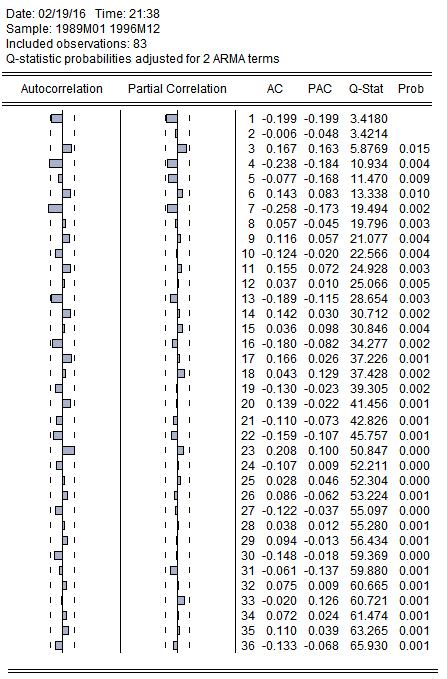
\includegraphics[width=0.8\linewidth]{imagenes/puros/modelo1-residuos-correlograma.png}
	\caption{Correlograma de los residuos del modelo ARIMA$(0,1,1)\times(0,1,1)_{12}$}
	\label{fig:modelo1-puros-residuos-correlograma}
\end{figure}

De forma similar, comprobamos que los residuos del modelo ARIMA$(2,1,0)\times(0,1,1)_{12}$ (Figuras~\ref{fig:modelo2-puros-residuos}~y~\ref{fig:modelo2-puros-residuos-correlograma}). 

\begin{figure}[tbph!]
	\centering
	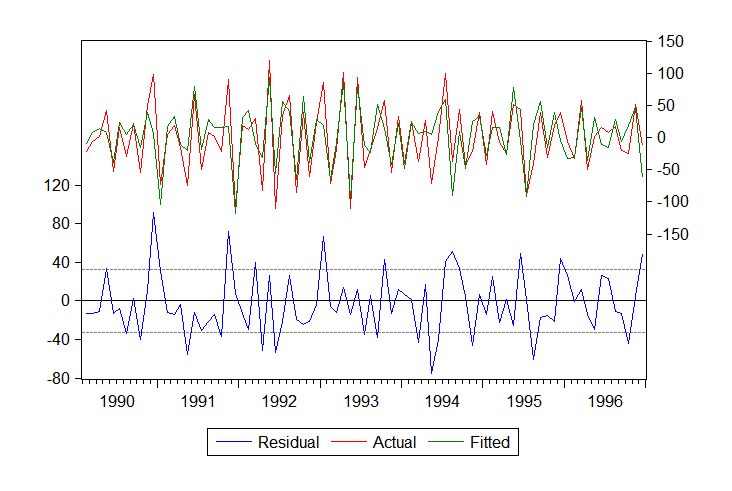
\includegraphics[width=0.8\linewidth]{imagenes/puros/modelo2-residuos.png}
	\caption{Residuos del modelo ARIMA$(2,1,0)\times(0,1,1)_{12}$}
	\label{fig:modelo2-puros-residuos}
\end{figure}

\begin{figure}[tbph!]
	\centering
	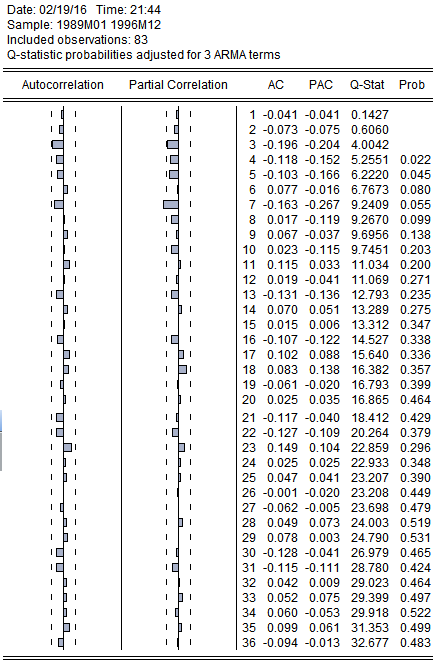
\includegraphics[width=0.8\linewidth]{imagenes/puros/modelo2-residuos-correlograma.png}
	\caption{Correlograma de los residuos del modelo ARIMA$(2,1,0)\times(0,1,1)_{12}$}
	\label{fig:modelo2-puros-residuos-correlograma}
\end{figure}

A tenor de los resultados, estamos ante dos modelos muy parecidos, pero nos decantaremos por el modelo ARIMA$(0,1,1)\times(0,1,1)_{12}$, ya que es el que menor valor tiene en los Akaike Info Criterion y Schwarz Criterion, aunque tiene un mayor error de regresión (cercano a 0.5).\\

Por tanto, la venta de puros viene dada por el modelo ARIMA$(2,1,0)\times(0,1,1)_{12}$.\\

Usaremos este modelo para predecir las ventas de puros en el año 1997. Estos datos se pueden ver en la Tabla~\ref{tbl:puros-predicciones}.\\

\begin{table}[htbp!]
	\centering
	\caption{Predicciones de ventas de puros para el año 1997}
	\label{tbl:puros-predicciones}
	\begin{tabular}{@{}cc@{}}
		\toprule
		\textbf{Mes} & \textbf{Predicción} \\ \midrule
		Enero             & $278.693$          \\
		Febrero           & $252.391$          \\
		Marzo             & $328.391$          \\
		Abril             & $301.391$          \\
		Mayo              & $306.391$          \\
		Junio             & $341.391$          \\
		Julio             & $279.391$          \\
		Agosto            & $320.391$          \\
		Septiembre        & $318.391$          \\
		Octubre           & $352.391$          \\
		Noviembre         & $304.391$          \\
		Diciembre         & $228.391$          \\ \bottomrule
	\end{tabular}
\end{table}

De forma más gráfica, se puede ver en la Figura~\ref{fig:puros-predicciones-1997}. Si comparamos la serie temporal inicial junto con las predicciones, observamos la clara tendencia descendente que se mantiene en el año 1997 (Figura~\ref{fig:puros-predicciones}).\\

\begin{figure}[tbph!]
	\centering
	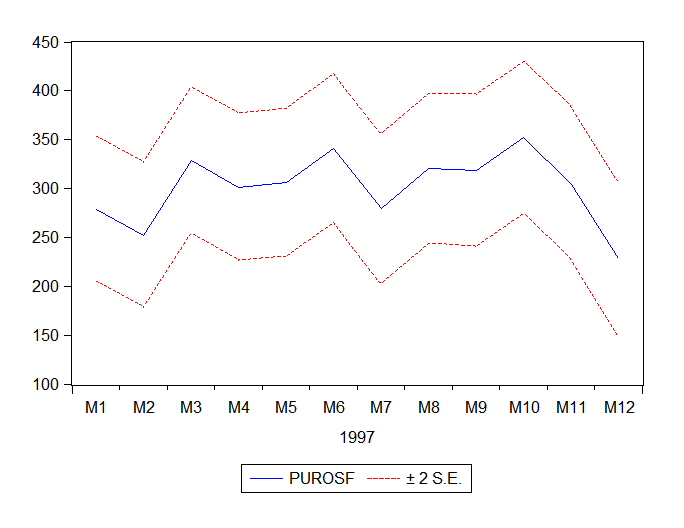
\includegraphics[width=0.8\linewidth]{imagenes/puros/puros-predicciones-1997.png}
	\caption{Predicciones (e intervalo de confianza) de ventas de puros para el año 1997}
	\label{fig:puros-predicciones-1997}
\end{figure}

\begin{figure}[tbph!]
	\centering
	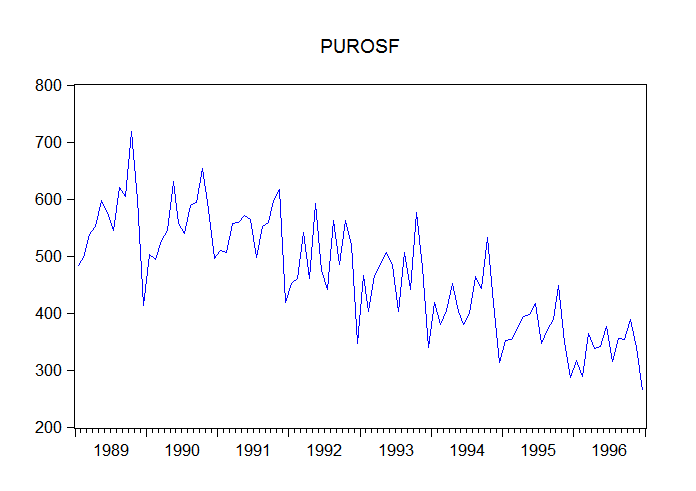
\includegraphics[width=0.8\linewidth]{imagenes/puros/puros-predicciones.png}
	\caption{Serie temporal de puros junto a las predicciones para el año 1997}
	\label{fig:puros-predicciones}
\end{figure}


\clearpage
\section{Conclusiones}
En este trabajo hemos visto cómo aplicar la metodología Box-Jenkins para modelizar distintas series temporales, que trataban distintos temas socioeconómicos: la primera serie era sobre el índice de paro de un país, y la segunda, la venta de puros. En ambos casos, hemos utilizado el software EViews, que gracias a su potencia y sus modelos de series temporales ya implementados, ha permitido ahorrar mucho tiempo estimando, analizando y prediciendo nuestros modelos propuestos.

\clearpage
\section{Código EViews}

A continuación se muestra el código EViews utilizado para resolver cada una de las series temporales planteadas.

\subsection{Índice de empleo}

\begin{verbatim}
empleo.sheet
{%graph}.line
empleo.correl(16)
series d
series dempleo = empleo - empleo(-1)
dempleo.sheet
{%graph}.line
dempleo.correl
{%equation}.ls(optmethod=opg) d(empleo,1) ar(1)
{%equation}.resids(g)
{%equation}.correl
{%equation}.ls(optmethod=opg) d(empleo,1) ma(1) ma(2)
{%equation}.resids(g)
{%equation}.results
{%equation}.correl
{%equation}.resids(g)
dempleo.hist
{%graph}.line
{%equation}.ls(optmethod=opg) d(empleo,1) ar(1)
smpl 1994q1 1994q4
{%equation}.forecast(e, g) empleof
smpl 1962q1 1993q4
{%equation}.forecast 
{%equation}.results
empleof.sheet
{%graph}.line
empleo.correl(16)
empleo.sheet
empleof.sheet
\end{verbatim}

\subsection{Venta de puros}


\begin{verbatim}
puros.sheet
{%graph}.line
puros.correl
series dpuros = puros - puros(-1)
dpuros.sheet
{%graph}.line
dpuros.correl
series dd12puros = dpuros(puros,1,12)
series dd12puros = d(puros,1,12)
dd12puros.sheet
{%graph}.line
dd12puros.correl
{%equation}.ls(optmethod=opg) dd12puros ma(1) sma(12)
{%equation}.ls(optmethod=opg) d(puros,1,12) ma(1) sma(12)
{%equation}.correl
{%equation}.resids(g)
{%equation}.correl
{%equation}.ls(optmethod=opg) d(puros,1,12) ar(1) ar(2) ma(12)
{%equation}.resids(g)
{%equation}.correl
{%equation}.ls(optmethod=opg) d(puros,1,12) ma(1) sma(1)
dd12puros.sheet
puros.sheet
pagestruct(end=1997M12)
smpl 1997m01 1997m12
{%equation}.forecast(e, g) purosf
smpl 1989m01 1996m12
purosf.sheet
{%graph}.line
\end{verbatim}

\end{document} 